\tikzset{every picture/.style={line width=0.75pt}} %set default line width to 0.75pt        

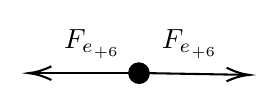
\begin{tikzpicture}[x=0.75pt,y=0.75pt,yscale=-1,xscale=1]
%uncomment if require: \path (0,300); %set diagram left start at 0, and has height of 300

%Shape: Circle [id:dp14447258656558515] 
\draw  [color={rgb, 255:red, 0; green, 0; blue, 0 }  ,draw opacity=1 ][fill={rgb, 255:red, 0; green, 0; blue, 0 }  ,fill opacity=1 ] (109.65,155.72) .. controls (109.6,153.11) and (111.68,151) .. (114.29,151) .. controls (116.9,151) and (119.05,153.11) .. (119.09,155.72) .. controls (119.14,158.33) and (117.06,160.45) .. (114.45,160.45) .. controls (111.84,160.45) and (109.69,158.33) .. (109.65,155.72) -- cycle ;
%Shape: Boxed Line [id:dp7138136373100961] 
\draw    (109.65,155.72) -- (63.24,155.72) ;
\draw [shift={(61.24,155.72)}, rotate = 360] [color={rgb, 255:red, 0; green, 0; blue, 0 }  ][line width=0.75]    (10.93,-3.29) .. controls (6.95,-1.4) and (3.31,-0.3) .. (0,0) .. controls (3.31,0.3) and (6.95,1.4) .. (10.93,3.29)   ;
%Shape: Boxed Line [id:dp010290116801451976] 
\draw    (119.09,155.72) -- (165.49,156.53) ;
\draw [shift={(167.49,156.57)}, rotate = 181] [color={rgb, 255:red, 0; green, 0; blue, 0 }  ][line width=0.75]    (10.93,-3.29) .. controls (6.95,-1.4) and (3.31,-0.3) .. (0,0) .. controls (3.31,0.3) and (6.95,1.4) .. (10.93,3.29)   ;

% Text Node
\draw (153.88,141.92) node [anchor=east] [inner sep=0.75pt]    {${F_{e}}_{_{+6}}$};
% Text Node
\draw (106.88,141.92) node [anchor=east] [inner sep=0.75pt]    {${F_{e}}_{_{+6}}$};


\end{tikzpicture}
